\lab{NumPy and SciPy}{NumPy and SciPy} 
\objective{Create and manipulate NumPy arrays and learn features available in NumPy and SciPy.}
\label{lab:NumPyArrays}

\section*{Introduction}

NumPy and SciPy\footnote{SciPy is also the name of a Python coding environment that includes the NumPy and SciPy libraries, as well as IPython, matplotlib, and other tools.} 
are the two Python libraries most used for scientific computing. 
NumPy is a package for manipulating vectors and arrays, and SciPy is a higher-level library built on NumPy. 
The basic object in NumPy is the \emph{array}, which is conceptually similar to a matrix. 
However, unlike a matrix, which has two dimensions, a NumPy \li{array} can have arbitrarily many dimensions. 
NumPy is optimized for fast array computations.

The convention is to import NumPy as follows.

\begin{lstlisting}
>>> import numpy as np
\end{lstlisting}

\section*{Learning NumPy}
The strategies discussed in the section ``Learning Python'' of Lab \ref{lab:Essential_Python} will also help you learn NumPy and SciPy. 
The following online resources are specific to SciPy:
\begin{itemize}
\item Official SciPy Documentation (\url{http://docs.scipy.org/doc/})
\item Sections 1.3 and 1.5 of the SciPy Lecture Notes (\url{http://scipy-lectures.github.io/})
\end{itemize}
The remainder of this lab is a brief summary of the tools available in NumPy and SciPy, beginning with NumPy arrays.


%%%%%%%%%%%%%%%%%%%%%%%%%%%%%%%%%%%%%%%%%%%%%%%%%%%%%%%%%%%
%%%%%%%%%%%%%%%%%%%%%%%%%%%%%%%%%%%%%%%%%%%%%%%%%%%%%%%%%%%
%%%%%%%%%%%%%%%%%%%%%%%%%%%%%%%%%%%%%%%%%%%%%%%%%%%%%%%%%%%
%%%%%%%%%%%%%%%%%%%%%%%%%%%%%%%%%%%%%%%%%%%%%%%%%%%%%%%%%%%
\section*{Arrays}

Conceptually, a 1-dimensional array (called a 1-D array) is just a list of numbers. 
An $n$-dimensional array (or $n$-D array) is an array of $(n-1)$-dimensional arrays. 
Thus, any 2-D array is conceptually a matrix, and a 3-D array is a list of matrices, which can be visualized as a cube of numbers. 
Each dimension is called an \emph{axis}. 
When a 2-D array is printed to the screen, the 0-axis indexes the rows and the 1-axis indexes the columns.

The NumPy array class is called \li{ndarray}. 
The simplest way to create an \li{ndarray} is to define it explicitly using nested lists.
\begin{lstlisting}
# Create a 1-D array.
>>> np.array([0, 3, 8, 6, 3.14])
array([0, 3, 8, 6, 3.14]) 

# Create a 2-D array.
>>> ex1 = np.array([[1, 1, 2], [3, 3, 4]])
>>> ex1
array([[1, 1, 2],
       [3, 3, 4]])

\end{lstlisting} 

You can view the length of each dimension with the \li{shape} command, and change the shape of an array with the \li{np.reshape()} function. 
The number of arguments passed to \li{reshape} tells NumPy the dimension of the new array, and the arguments specify the length of each dimension. 
An argument of \li{-1} tells NumPy to make that dimension as long as necessary.
\begin{lstlisting}
# The 0-axis of ex1 has length 2.
>>> ex1.shape
(2, 3)
>>> ex1.reshape(3, 2)
array([[1, 1],
       [2, 3],
       [3, 4]])

# Fill the 0-axis.
>>> ex1.reshape(-1)
array([1, 1, 2, 3, 3, 4])
# If we know we want two columns, but don't know how many rows will result.
>>> ex1.reshape(-1, 2)
array([[1, 1],
      [2, 3],
      [3, 4]])
\end{lstlisting}

Array objects also support the usual binary operators, including addition \li{+} and element-wise multiplication \li{*}. For Python lists, the \li{+} operator performs concantenation and the \li{*} operator is not defined.

\begin{lstlisting}
>>> a = [1,2,3]
>>> b = [4,5,6]
>>> a+b
[1, 2, 3, 4, 5, 6]
>>> a*b
TypeError: cannot multiply sequence by non-int of type 'list'

>>> a = np.array(a)
>>> b = np.array(b)
>>> a+b
array([5,7,9])
>>> a*b
array([4, 10, 18])
\end{lstlisting}


%%%%%%%%%%%%%%%%%%%%%%%%%%%%%%%%%%%%%%%%%%%%%%%%%%%%%%%%%%%
\subsection*{Why Use Arrays?}
NumPy arrays are drastically more efficient than nested Python lists for large computations. 
In this section we will compare matrix multiplication in Python and in NumPy.

\begin{problem}
A matrix in NumPy is just a 2-D array. Given matrices $A$ and $B$, there are two different ways we can perform matrix multiplication. We can use \li{np.dot(A,B)} or \li{A.dot(B)}. 

Perform the matrix multiplication $A * B$ on the following matrices:
\begin{center}
$A = \begin{bmatrix} 2&4&0 \\ -3&1&-1 \\ 0&3&2 \end{bmatrix}$
$B = \begin{bmatrix} 3&-1&2 \\ -2&-3&0 \\ 1&0&-2 \end{bmatrix}$
\end{center}
Remember that to be able to use \li{np.dot}, we must first define $A$ and $B$ as NumPy arrays.
\label{prob:multiply_problem}
\end{problem}



%\begin{problem}\label{prob:multiply_problem}
%A matrix in NumPy is just a 2-D array. How can you multiply two 2-D NumPy arrays as matrices? 
%Hint: Use the strategies outlined in the section ``Learning NumPy''.
%\end{problem}

After doing the previous problem, you should know how to implement matrix multiplication in NumPy. 
On the other hand, a matrix in Python can be represented as a list of lists.  We can perform matrix multiplication using lists by using numerical multiplication and addition. 
The following function will multiply two such matrices in this manner in Python without using NumPy.

\lstinputlisting[style=fromfile]{arr_mult.py}

Table \ref{table:square_times} documents how long\footnote{You can replicate this experiment yourself. In IPython, you can find the execution time of a line of code by prefacing it with \li{\%timeit}. 
If you aren't using IPython, you will need
to use the timeit function documented here: \url{https://docs.python.org/2/library/timeit.html}.} 
one computer took to square a $k \times k$ matrix in both Python (using the function \li{arr_mult}) and NumPy (using the method you found in Problem \ref{prob:multiply_problem}) for various values of $k$. 
As you can see, NumPy is much faster. One reason for this is that algorithms in NumPy are usually implemented in C or in Fortran. 

\begin{table}
 \begin{tabular}{|c|l|l|} \hline Data Structure & $k\times k$ & Time (s) \\ \hline 
 Python List  	& $10\times10$ 	& 0.0002758503 \\ 
 \cline{2-3} 	& $100\times100$ 	& 0.1336028576 \\ 
 \cline{2-3} 	& $1000\times1000$ & 200.4009799957 \\ 
 %& $1\times1$ 		& 0.0000181198 \\ 
\hline \hline 
 NumPy Array 	& $10\times10$ 	& 0.0000109673 \\
 \cline{2-3} 	& $100\times100$ 	& 0.0009210110 \\ 
 \cline{2-3} 	& $1000\times1000$ & 2.1682999134 \\
 %& $1\times1$ 		& 0.0000298023 \\ 
 \hline \end{tabular}
 \caption{Time for one computer to square a $k \times k$ matrix in Python and NumPy.}
\label{table:square_times} 
\end{table}
 
 
% 



%%%%%%%%%%%%%%%%%%%%%%%%%%%%%%%%%%%%%%%%%%%%%%%%%%%%%%%%%%%
\subsection*{Data Types}
Unlike Python containers, a NumPy array requires that all of its elements have the same data type. 
The data types used by NumPy arrays are machine-native and avoid the overhead of Python objects, meaning that they are faster to compute with. 
A NumPy \li{int} and a Python \li{int} are not the same; the former has been optimized to speed up numerical computations. 
Datatypes supported by NumPy are shown in Table \ref{table:numpytypes}.

\begin{table}
\begin{tabular}{l|l} 
Data type & Description 
\\ \hline 
\li{bool} & Boolean \\ 
\li{int8} & 8-bit integer \\ 
\li{int16} & 16-bit integer \\ 
\li{int32} & 32-bit integer \\
\li{int64} & 64-bit integer \\ 
\li{int} & Platform integer (depends on platform) \\ 
\li{uint8} & Unsigned 8-bit integer \\ 
\li{uint16} & Unsigned 16-bit integer \\ 
\li{uint32} & Unsigned 32-bit integer \\
\li{uint64} & Unsigned 64-bit integer \\ 
\li{float16} & Half-precision float \\ 
\li{float32} & Single-precision float \\ 
\li{float64} & Double-precision float (also \li{float}) \\ 
\li{complex64} & Complex number represented by two single-precision floats \\ 
\li{complex128} & Complex number represented by two double-precision floats (also \li{complex})
\end{tabular} 
\caption{Native numerical data types available in NumPy.}
\label{table:numpytypes} 
\end{table} 

Here is an example of how to manipulate data types in NumPy:
\begin{lstlisting}
# Access the data type of an array.
>>> ex2 = np.array(range(5))
>>> ex2.dtype
dtype('int64')

# Specify the data type of an array.
>>> ex3 = np.array(range(5), dtype=np.float)
>>> ex3.dtype
dtype('float64')
\end{lstlisting}

%%%%%%%%%%%%%%%%%%%%%%%%%%%%%%%%%%%%%%%%%%%%%%%%%%%%%%%%%%%
\subsection*{Creating Arrays}
In addition to \li{np.array()}, NumPy provides efficient ways to create special kinds of arrays. The function \li{np.arange([start], stop, [step])} returns an array of numbers from \li{start} up to, but not including, \li{stop}. Like other functions with similar parameters, \li{start} defaults to $0$ and \li{step} defaults to $1$. 

\begin{lstlisting}
>>> np.arange(5)
array([0,1,2,3,4])
>>> np.arange(10, 20, 2) 
array([10, 12, 14, 16, 18])
\end{lstlisting}

Use \li{np.linspace(start, stop, num=50)} to create an array of \li{num} numbers evenly spaced in the interval from \li{start} to \li{stop} inclusive.
\begin{lstlisting}
>>> np.linspace(0, 32, 4) 
array([  0.        ,  10.66666667,  21.33333333,  32.        ])
\end{lstlisting} 

We can even create arrays of random values chosen
from probability distributions. These probability distributions are stored
in the submodule \li{np.random}. 
\begin{lstlisting}
>>> np.random.rand(5) # Returns uniformly distributed values in [0, 1).
array([ 0.21845499,  0.73352537,  0.28064456,  0.66878454,  0.44138609])
\end{lstlisting} 
Some other commonly-used functions are \li{np.random.randn}, which samples from the normal distribution, \li{np.random.randint}, which randomly selects integers from a range, and \li{np.random.random_integers} which returns an array of random integers in a given range.  
There are many functions for creating arrays besides these, some of which are described in Table \ref{table:numpycreate}. 
See \url{http://docs.scipy.org/doc/numpy/reference/routines.array-creation.html} for more details.

\begin{table}
\begin{tabular}{l|l} 
Function & Description 
\\ \hline 
\li{diag} & Extract a diagonal or construct a diagonal array.\\
\li{empty} & Return a new array of given shape and type, without initializing entries. \\ 
\li{empty_like} & Return a new array with the same shape and type as a given array. \\
\li{eye} & Return a 2-D array with ones on the diagonal and zeros elsewhere. \\ 
\li{identity} & Return the identity array. \\ 
\li{meshgrid} & Return coordinate matrices from two coordinate vectors.\\ 
\li{ones} & Return a new array of given shape and type, filled with ones. \\ 
\li{ones_like} & Return an array of ones with the same shape and type as a given array. \\ 
\li{zeros} & Return a new array of given shape and type, filled with zeros. \\ 
\li{zeros_like} & Return an array of zeros with the same shape and type as a given array. \\ 
\end{tabular} 
\caption{Some functions for creating arrays in NumPy.}
\label{table:numpycreate} 
\end{table} 


%%%%%%%%%%%%%%%%%%%%%%%%%%%%%%%%%%%%%%%%%%%%%%%%%%%%%%%
\subsection*{Indexing and Slicing} 
Indexing for a 1-D NumPy array works exactly like indexing for a Python list. 
To access a single entry of a multi-dimenional array, say a 3-D array, you should use the syntax \li{f[i, j, k]}. 
While the syntax \li{f[i][j][k]} will also work, it is significantly slower because each bracket returns an array slice. 
Similarly, slicing an array works just like slicing a list, but with more dimensions. Using a single colon as an argument extracts everything in the specified axis.
\begin{lstlisting}
>>> ex4 = np.arange(25).reshape((5,5)) 
>>> ex4
array([[ 0,  1,  2,  3,  4],
       [ 5,  6,  7,  8,  9],
       [10, 11, 12, 13, 14],
       [15, 16, 17, 18, 19],
       [20, 21, 22, 23, 24]])
>>> ex4[4, -2]
23

# Extract the lower right 2x2 subarray.
>>> ex4[3:, 3:] 
array([[18, 19],
       [23, 24]])
       
# Extract the second column. The returned array is 1-D.
>>> ex4[:, 1] 
array([ 1,  6, 11, 16, 21]) 

# Reverse the order of the columns.
>>> ex4[:, ::-1] 
array([[ 4,  3,  2,  1,  0],
       [ 9,  8,  7,  6,  5],
       [14, 13, 12, 11, 10],
       [19, 18, 17, 16, 15],
       [24, 23, 22, 21, 20]])
\end{lstlisting}

\subsection*{Fancy Indexing}
Fancy indexing is a second way to access elements of an array. 
There are two types of fancy indexing: boolean and integer. 
Boolean indexing uses an array of \li{True} or \li{False} values to 
determine which elements of the array to take. 

%np.argsort
\begin{lstlisting}
>>> my_array = np.array([0, 10, 20, 30, 40])
>>> bool_mask = np.array([1,0,1,1,0], dtype=bool)
>>> my_array[bool_mask]
array([0,20,30])

# Return only the values larger than 25.
>>> comparision_mask = my_array > 25
>>> comparision_mask
array([False, False, False, True, True], dtype=bool)
>>> my_array[comparison_mask]
array([30, 40])

# If we do not need to save the mask for other uses, we can achieve the same result by doing the following:
>>> my_array[my_array>25]
array([30, 40])

# np.argsort returns a list of indices that would sort an array.
>>> my_array = np.array([4,1,6,3,7,2,5])
>>> mask = np.argsort(my_array)
>>> my_array[mask]
array([1, 2, 3, 4, 5, 6, 7])
\end{lstlisting}

Integer indexing uses Python lists to determine what array values to access.
\begin{lstlisting}
>>> my_array = np.array([0,10,20,30,40])
>>> int_mask = [2,3,1]
>>> my_array[int_mask]
array([20,30,10])
\end{lstlisting}

Fancy indexing can
be used for assignment. For example, we can set all values of an array
that are less than \li{25} to \li{0} in the following way:
\begin{lstlisting} 
>>> my_array[my_array<25] = 0
>>> my_array
array([0, 0, 0, 30, 40])
\end{lstlisting}

\begin{problem}
Write a function that accepts an array and returns an array with all nonnegative numbers. If an entry in the inputed array is negative, set it to $0$. Though one of your first instincts may be to use a \li{for} loop, it is much more efficient to solve this problem using fancy indexing.
\end{problem}

%%%%%%%%%%%%%%%%%%%%%%%%%%%%%%%%%%%%%%%%%%%%%%%%%%%%%%%
\subsection*{Array Views and Copies} 
NumPy has two ways of returning an array. Slice operations and indexing always return
a \emph{view} and fancy indexing always returns a \emph{copy}.
Understand that even though they may look the same, views and copies are different.


A view of an array is a distinct object from the original array in Python, but it references the same place in memory. 
Thus, when you change elements in a view, you also change the array it references.
\begin{lstlisting}
>>> ex5 = np.arange(5)

# Slicing produces a view of ex5. 
>>> view_ex5 = ex5[:]
>>> view_ex5

# Check that ex5 and view_ex5 are distinct objects in Python.
>>> id(view_ex5) == id(ex5) 
False

# Change the third element of view_ex5 to 500
# Changing view_ex5 also changes ex5.
>>> view_ex5[2] = 500 
>>> view_ex5
array([  0,   1, 500,   3,   4])
>>> ex5 
array([  0,   1, 500,   3,   4])
\end{lstlisting} 

A copy of an array is a separate array with its own place in memory. 
Thus, when you change a copy of an array, you do not affect the original array. 
Because copying an array uses more memory and also more time, it should only be done when necessary. 
An array can be copied using the \li{np.copy()} function (also available as a method of 
the array object, for example \li{my_array.copy()} returns a copy of \li{my_array}). 

\begin{lstlisting}
>>> copy_ex5 = np.copy(ex5) 

# Check that ex5 and copy_ex5 are distinct objects in Python.
>>> id(copy_ex5) == id(ex5) 
False

# Change the third element of copy_ex5 to 1000
# Changing copy_ex5 does not affect ex5.
>>> copy_ex5[2] = 1000 
>>> copy_ex5
array([  0,   1, 1000,   3,   4])
>>> ex5
array([  0,   1, 500,   3,   4])
\end{lstlisting} 

Whenever possible, the function \li{np.reshape()} returns a view. 
See the documentation for more information. 



%%%%%%%%%%%%%%%%%%%%%%%%%%%%%%%%%%%%%%%%%%%%%%%%%%%%%
\section*{More Methods of NumPy Arrays} 
Some of the more common methods of NumPy arrays are described in Table \ref{table:ndarraymethods}. 
A more comprehensive list can be found at
\url{http://docs.scipy.org/doc/numpy/reference/generated/numpy.ndarray.
html}.

\begin{table}
\centering 
\begin{tabular}{l|p{10cm}}
    \hline
    Function & Description \\
    \hline
    \li{all} & returns True if all elements evaluate to True \\
    \li{any} & returns True if any elements evaluate to True \\
    \li{argmax} & indices of maximum value(s) \\
    \li{argmin} & indices of minimum value(s) \\
    \li{argsort} & indices that would sort the array \\
    \li{astype} & casts a copy of an array to a different data type \\
    \li{clip} & restrict values in an array to fit within a given range\\
    \li{conj} & return the complex conjugate of the array \\
    \li{copy} & return a copy of the array\\
    \li{diagonal} & return a given diagonal of the array \\
    \li{dot} & matrix multiplication \\
    \li{max} & max element of the array \\
    \li{mean} & average of the array \\
    \li{min} & minimum element of the array \\
    \li{prod} & product of elements of the array \\
    \li{ravel} & make a flattened version of an array, return a view if
    possible \\
    \li{reshape} & return a view of the array with a changed shape \\
    \li{round} & return a rounded version of the array \\
    \li{sort} & sort the array in place \\
    \li{std} & compute the standard deviation \\
    \li{sum} & sum the elements of the array \\
    \li{swapaxes} & return a view with the given axes swapped \\
    \li{tolist} & return the array represented as a list or nested list\\
    \li{trace} & return the sum of the elements along the main diagonal\\
    \li{var} & return the variance of the array \\
    \li{vstack} & stack arrays in sequence vertically \\
    \hline
    \end{tabular} \caption{A few of the methods of NumPy arrays.}
    \label{table:ndarraymethods} \end{table}

Many of these methods have the option to operate \emph{along an axis}. 
When called in this way on an $n$-D array, these methods return an $(n-1)$-D array (the specified axis is collapsed in the evaluation process).

\begin{lstlisting}
>>> ex6 = np.arange(9).reshape(3, 3)
>>> ex6
array([[0, 1, 2],
       [3, 4, 5],
       [6, 7, 8]])
       
# Return the maximum value in the array
>>> ex6.max() 
8

# Return the maximum values evaluated along the 0-axis
>>> ex6.max(axis=0)
array([6, 7, 8])

# Return the maximum values evaluated along the 1-axis
>>> ex6.max(axis=1)
array([2, 5, 8])
\end{lstlisting}


\begin{problem}
% There should be more problems like this in the vectorization lab. I'll
% include this one here for now though.
Write a function which accepts an integer $n$ as input and does the following:
\begin{enumerate}
\item Creates an $n\times n$ array of \li{floats} randomly chosen from a normal distribution.
\item Computes the mean of each row (use a built-in command).
\item Computes the variance of these means (use a built-in command).
\end{enumerate}
As you increase $n$, what happens to the output of 
your function? This illustrates one version of
the Law of Large Numbers, about which you will learn more later on.
\end{problem}

\begin{problem} 
One good application of array slicing is the Jacobi
method for solving Laplace's equation, which is used to model
steady-state heat flow on a square. This problem will help you implement the Jacobi method.

Make a function that accepts an array and a float (which represents a tolerance) as input and does the
following: 
\begin{enumerate}
\item Makes a copy of the array. 
\item Creates a variable to track the difference between the arrays. Initialize
it as the tolerance parameter your function accepts. 
\item While the difference is greater than or equal
to the tolerance 
\begin{enumerate} 
\item Sets all points that are not on an edge of the new array equal to the average of their 4 immediate neighbors. 
Use the values from the old array for this computation. 
This should only take one line and should be based entirely on array slicing, NOT iterating through the array.
(Hint: given a 2D array \li{A}, the slice \li{A[1:-1,1:-1]} references
all non-edge entries, \li{A[:-2,1:-1]} references the upper neighbors,
and \li{A[1:-1,2:]} references the right neighbors.) 
\item Updates the difference to be the maximum of the absolute value of the new array
minus the old one. 
\item Copies the values from the new array into the old
one (without creating a new array). 
\end{enumerate} 
\end{enumerate}

Now use the following code to generate a plot of your results.
\lstinputlisting[style=fromfile]{laplace_plot.py} 
It should resemble the following figure.

\begin{figure} [H]
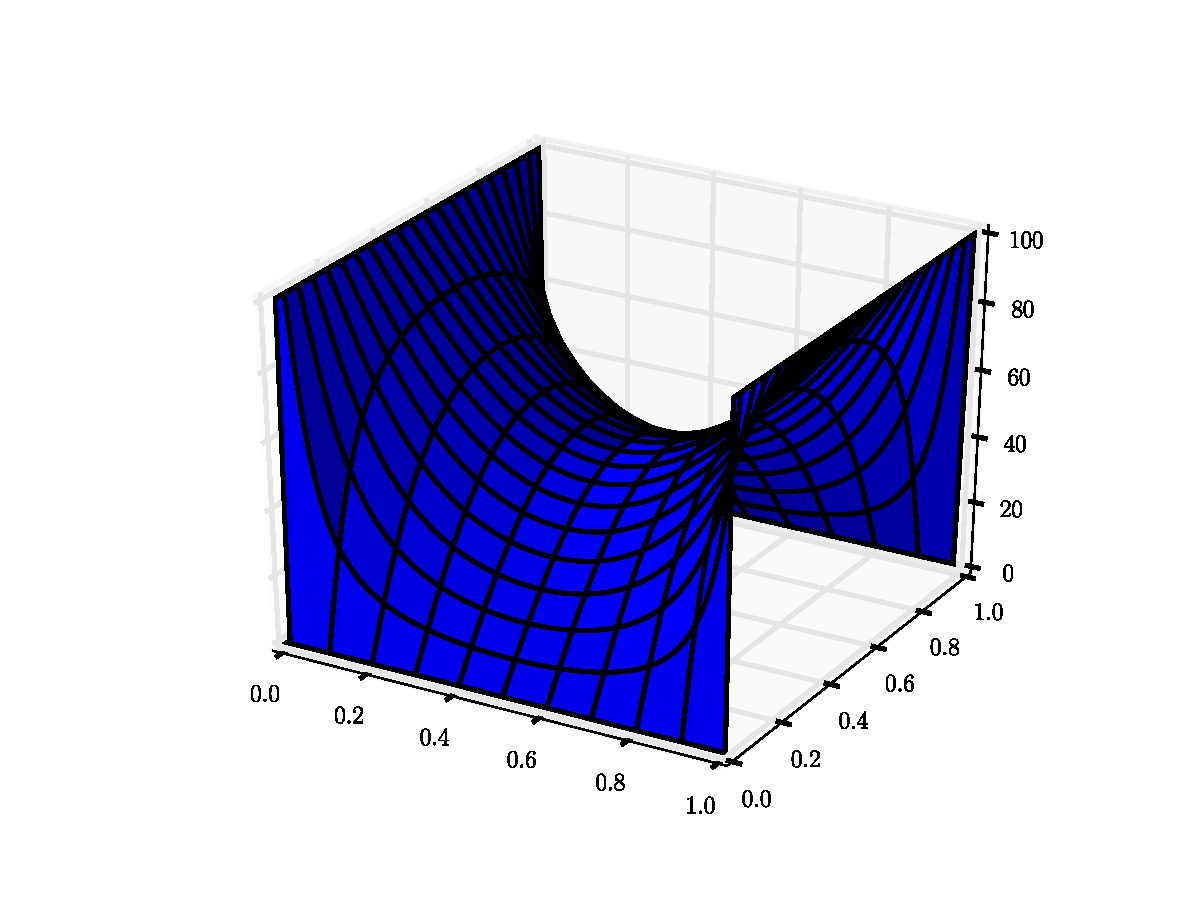
\includegraphics[width=.75\textwidth]{laplace.pdf}
\end{figure} 
\end{problem}

\subsection*{Iterating Through Arrays}

Iterating through an array negates most speed advantages of NumPy. 
You should avoid doing this whenever possible.
You can often avoid iterating through arrays by using \emph{array broadcasting} and \emph{universal functions}, discussed in the next section.

It is occasionally valid to iterate through an array. 
The function \li{np.nditer()} will create an object that iterates through an array as quickly as possible.


\section*{NumPy and SciPy}
We now introduce some additional features of NumPy and SciPy.

\subsection*{Array Broadcasting}
Many matrix operations make sense only when the two operands have the same shape. 
Two examples are addition and element-wise multiplication. 
Broadcasting is NumPy's way of extending such operations to accept some (not all) operands with different shapes. 
Broadcasting happens automatically whenever it is necessary. 

To understand broadcasting, let us look at an example. 
\begin{lstlisting}
>>> A = np.ones(3);
>>> A
array([ 1.,  1.,  1.])
>>> B = np.vstack([1, 2, 3])
>>> B
array([[1],
       [2],
       [3]])
>>> A+B
array([[ 2.,  2.,  2.],
       [ 3.,  3.,  3.],
       [ 4.,  4.,  4.]])
\end{lstlisting}
We will now describe the algorithm used to obtain the result for \li{A+B} above. 
First, the shapes of \li{A} and \li{B} are lined up, starting at the far right, and 1's are prepended to the shorter tuple. So
\begin{lstlisting}
A 	(1-D array):     3
B	(2-D array): 3 x 1
\end{lstlisting}
becomes
\begin{lstlisting}
A 	(1-D array): 1 x 3
B	(2-D array): 3 x 1
\end{lstlisting}
For broadcasting to work, the dimensions must be compatible; that is, in a given axis, the lengths are equal, or one of the lengths is 1. 
Second, the arrays \li{A} and \li{B} are ``stretched'' one axis at a time until the lengths of their axes are the same. 
In each axis, if the lengths are different, the smaller array is copied along that axis (or ``stretched''), until it is the size of the larger array. 
Conceptually, we are creating new $3 \times 3$ arrays $A'$ and $B'$ where
\[
A' = \left[ \begin{array}{ccc}
1 & 1 & 1\\
1 & 1 & 1\\
1 & 1 & 1 \end{array} \right] \qquad \text{and} \qquad B' =  \left[ \begin{array}{ccc}
1 & 1 & 1\\
2 & 2 & 2\\
3 & 3 & 3\end{array} \right].
\]
Finally, NumPy returns the sum $A'+B'$.

We emphasize that the ``stretching'' in this example is only conceptual, and no new array $A'$ or $B'$ is created. However, 
you should still be careful when broadcasting large arrays because you can fill the 
RAM on your computer, which can sometimes freeze the system.
For a more detailed description of array broadcasting rules, see 
\url{http://docs.scipy.org/doc/numpy/user/basics.broadcasting.html}.

\begin{problem}
Create a $100\times100\times3$ array of random integers taking values in the range 
[0, 255]. Such an array can represent an RGB image of $100\times100$ pixels, 
where each pixel is associated with an array of three integers indicating the 
amounts of red, green, and blue color present in that pixel.
Use array broadcasting to multiply the red and green values by $0.5$. 
(Such an operation would tone down the red and green colors and make the 
image appear more blue.) 

To visualize your solutions, you may use the following function.
\lstinputlisting[style=fromfile]{blue_shift_plot.py} 
\end{problem}

\subsection*{Universal Functions}

A universal function, or \li{ufunc}, operates on an array element-wise. 
It outputs an array of the same shape and datatype as the input array. 
Using a universal function is usually much faster than iterating through the array yourself.

Many scalar functions from the Python standard library have a universal analog that operates on arrays. 
For example, \li{math.sin()} operates on scalars, and \li{numpy.sin()} operates on arrays. 
If you have a simple operation that you want to perform element-wise on an array, you should see if SciPy has a universal function that will do it (it probably does). 
For a list of available \li{ufuncs}, see \url{http://docs.scipy.org/doc/numpy/reference/ufuncs.html#available-ufuncs}.

Most universal functions also allow you to specify an output array, which must have the same shape as the input array.
Doing so can reduce memory allocation. 

\begin{lstlisting}
>>> ex7 = np.arange(3, dtype=float)

# Take exp(ex7) and store the result in ex7.
>>> np.exp(ex7, out=ex7) 
>>> ex7
array([ 1.        ,  2.71828183,  7.3890561 ])
\end{lstlisting}

Although universal functions also accept scalar inputs, they can be much slower than the corresponding standard library function. 
Thus, use standard library functions on scalars and universal functions on arrays.

\subsection*{Linear Algebra}
Both NumPy and SciPy have a linear algebra library, but the SciPy library is larger. The SciPy linear algebra library is typically imported as follows:

\begin{lstlisting}
from scipy import linalg as la
\end{lstlisting}

The linear algebra library contains several functions to construct special 
matrices, located in 
\li{linalg.special_matrices}. There are also functions that will invert matrices, find determinants and norms, solve linear systems and least squares problems, and find special matrix decompositions. You can read more about the linear algebra capabilities of SciPy in the 
documentation for the \li{linalg} module found at
\url{http://docs.scipy.org/doc/scipy/reference/linalg.html}.

Finally, the \li{scipy.linalg} library has a \li{matrix} class that is very 
similar to a 2-D NumPy array. The matrix class can be convenient when doing matrix 
operations. However, in such situations we still recommend using NumPy arrrays, which have many of the same features and are also compatible with all other SciPy operations.

The \li{scipy.linalg} library will be essential for the remainder of the labs in this manual. We will address the details of this package at length in future labs. 

\begin{comment}
\subsection*{Polynomials}
The \li{np.poly1d} object represents a polynomial in NumPy. The constructor is called with the coefficients of the desired polynomial. 

\begin{lstlisting}
>>> poly_array = np.poly1d([3, 5, 1, 2, 0, 1])
>>> print poly_array
   5     4     3     2
3 x + 5 x + 1 x + 2 x + 1
\end{lstlisting}

The object \li{poly_array} represents the polynomial $3x^5+5x^4+x^3+2x^2+1$.
NumPy provides many functions to operate on \li{poly1d} objects (see \url{http://docs.scipy.org/doc/numpy/reference/routines.polynomials.polynomial.html}).



Here is an example using the \li{poly1d} class. Recall that
\[
e^x = \sum_{n=0}^{\infty} \frac{x^n}{n!}.
\]
The following function evaluates the $n^{th}$ partial sum of this series at the value $a$.

\lstinputlisting[style=fromfile]{exp.py}

The last two lines can be condensed by using the following command.

\begin{lstlisting}
np.polyval(p, a)
\end{lstlisting}

\begin{problem}
\leavevmode
\begin{enumerate}
\item Use NumPy's polynomial objects to approximate the following series.
\[
\arcsin x = \sum_{n=0}^{\infty} \frac{\left(2 n\right) ! x^{2 n + 1}}{\left(2 n + 1\right)\left(n!\right)^2 4^n}
\]
This series converges on $(-1, 1)$. Use your series approximation to approximate $\pi$. Hint: think of the powers of $x$ that
are not included in the series as having zero coefficients.

\item The lambert W function is the inverse of $x e^x$.
Its Taylor series is below (note the index starts at 1).
\[
W(x) = \sum_{n=1}^{\infty} \frac{\left(-n\right)^{n-1} x^n}{n!}
\]
This series has a radius of convergence of $\frac{1}{e}$.
Use the series to approximate a number $x$ such that $x e^x = \frac{1}{4}$.
Verify that your approximation is close.


\end{enumerate}
\end{problem}
\end{comment}

